\documentclass[tikz,border=2mm]{standalone}
\usepackage[T1]{fontenc}
\usepackage[utf8]{inputenc}
\usepackage{lmodern}
\usepackage[scaled=1]{helvet}
\renewcommand{\familydefault}{\sfdefault}
\usepackage{amssymb,textcomp}
\usepackage{sansmath}
\usetikzlibrary{arrows.meta,calc}
\renewcommand{\arraystretch}{1.15}
\setlength{\tabcolsep}{3pt}
\tikzset{
  Fs/.style={font=\fontsize{5.8}{7}\selectfont},
  Fn/.style={font=\fontsize{6.6}{8}\selectfont},
  Fb/.style={font=\fontsize{6.8}{8.2}\selectfont\bfseries},
  Ft/.style={font=\fontsize{9}{11}\selectfont\bfseries},
  enc/.style={densely dashed,line width=0.45pt},
  tag/.style={font=\fontsize{6.2}{7}\selectfont\bfseries,draw,rounded corners=1.5pt,fill=white,inner sep=1pt},
  % ---------------- símbolos IEC 60617 ----------------
  % módulo FV: rectángulo con diodo, centrado en el punto
  pics/fv/.style={code={
    \draw[fill=white] (-0.16,-0.15) rectangle (0.16,0.15);
    \draw (-0.09,0.08) -- (0.09,0.08) -- (0,-0.08) -- cycle;
    \draw (-0.09,-0.08) -- (0.09,-0.08);}},
  % interruptor automático horizontal de (0,0) a (0.8,0); la cuchilla sube
  pics/tm/.style={code={
    \draw (0,0) -- (0.16,0); \draw (0.16,0) -- (0.66,0.2); \draw (0.64,0) -- (0.8,0);
    \draw (0.59,-0.05) -- (0.69,0.05); \draw (0.59,0.05) -- (0.69,-0.05);}},
  % interruptor automático vertical de (0,0) a (0,-0.8); la cuchilla va a la izquierda
  pics/tmv/.style={code={
    \draw (0,0) -- (0,-0.16); \draw (0,-0.16) -- (-0.2,-0.66); \draw (0,-0.64) -- (0,-0.8);
    \draw (-0.05,-0.59) -- (0.05,-0.69); \draw (0.05,-0.59) -- (-0.05,-0.69);}},
  % tierra, conectada desde arriba en (0,0)
  pics/tierra/.style={code={
    \draw (0,0) -- (0,-0.12); \draw (-0.13,-0.12) -- (0.13,-0.12);
    \draw (-0.085,-0.17) -- (0.085,-0.17); \draw (-0.04,-0.22) -- (0.04,-0.22);}},
  % DPS conectado hacia abajo desde (0,0), con su tierra
  pics/dps/.style={code={
    \fill (0,0) circle (0.035); \draw (0,0) -- (0,-0.12);
    \draw (-0.1,-0.12) rectangle (0.1,-0.46);
    \draw[-{Stealth[length=1mm,width=0.9mm]}] (0,-0.16) -- (0,-0.42);
    \draw (0,-0.46) -- (0,-0.55); \pic at (0,-0.55) {tierra};}},
  % batería horizontal: entra por la izquierda en (0,0), placa larga (+) a la izquierda
  pics/bath/.style={code={
    \draw (0,0) -- (0.22,0); \draw[line width=0.8pt] (0.22,-0.18) -- (0.22,0.18);
    \draw[line width=1.8pt] (0.32,-0.09) -- (0.32,0.09); \draw (0.32,0) -- (0.54,0);
    \node[Fs,anchor=south] at (0.14,0.12) {+};}},
  % convertidor: cuadrado con diagonal (lado 1.0) centrado; #1 entrada, #2 salida
  pics/conv/.style 2 args={code={
    \draw[fill=white] (-0.5,-0.5) rectangle (0.5,0.5); \draw (-0.5,-0.5) -- (0.5,0.5);
    \node[Fn] at (-0.24,0.24) {#1}; \node[Fn] at (0.24,-0.24) {#2};}},
}
\newcommand{\cc}{\begin{tikzpicture}[baseline=-0.6ex]\draw (0,0.035)--(0.26,0.035);\draw[densely dashed] (0,-0.035)--(0.26,-0.035);\end{tikzpicture}}
\newcommand{\ca}{\begin{tikzpicture}[baseline=-0.6ex]\draw plot[domain=0:1,samples=20,smooth] ({0.26*\x},{0.05*sin(360*\x)});\end{tikzpicture}}
\begin{document}
\sansmath
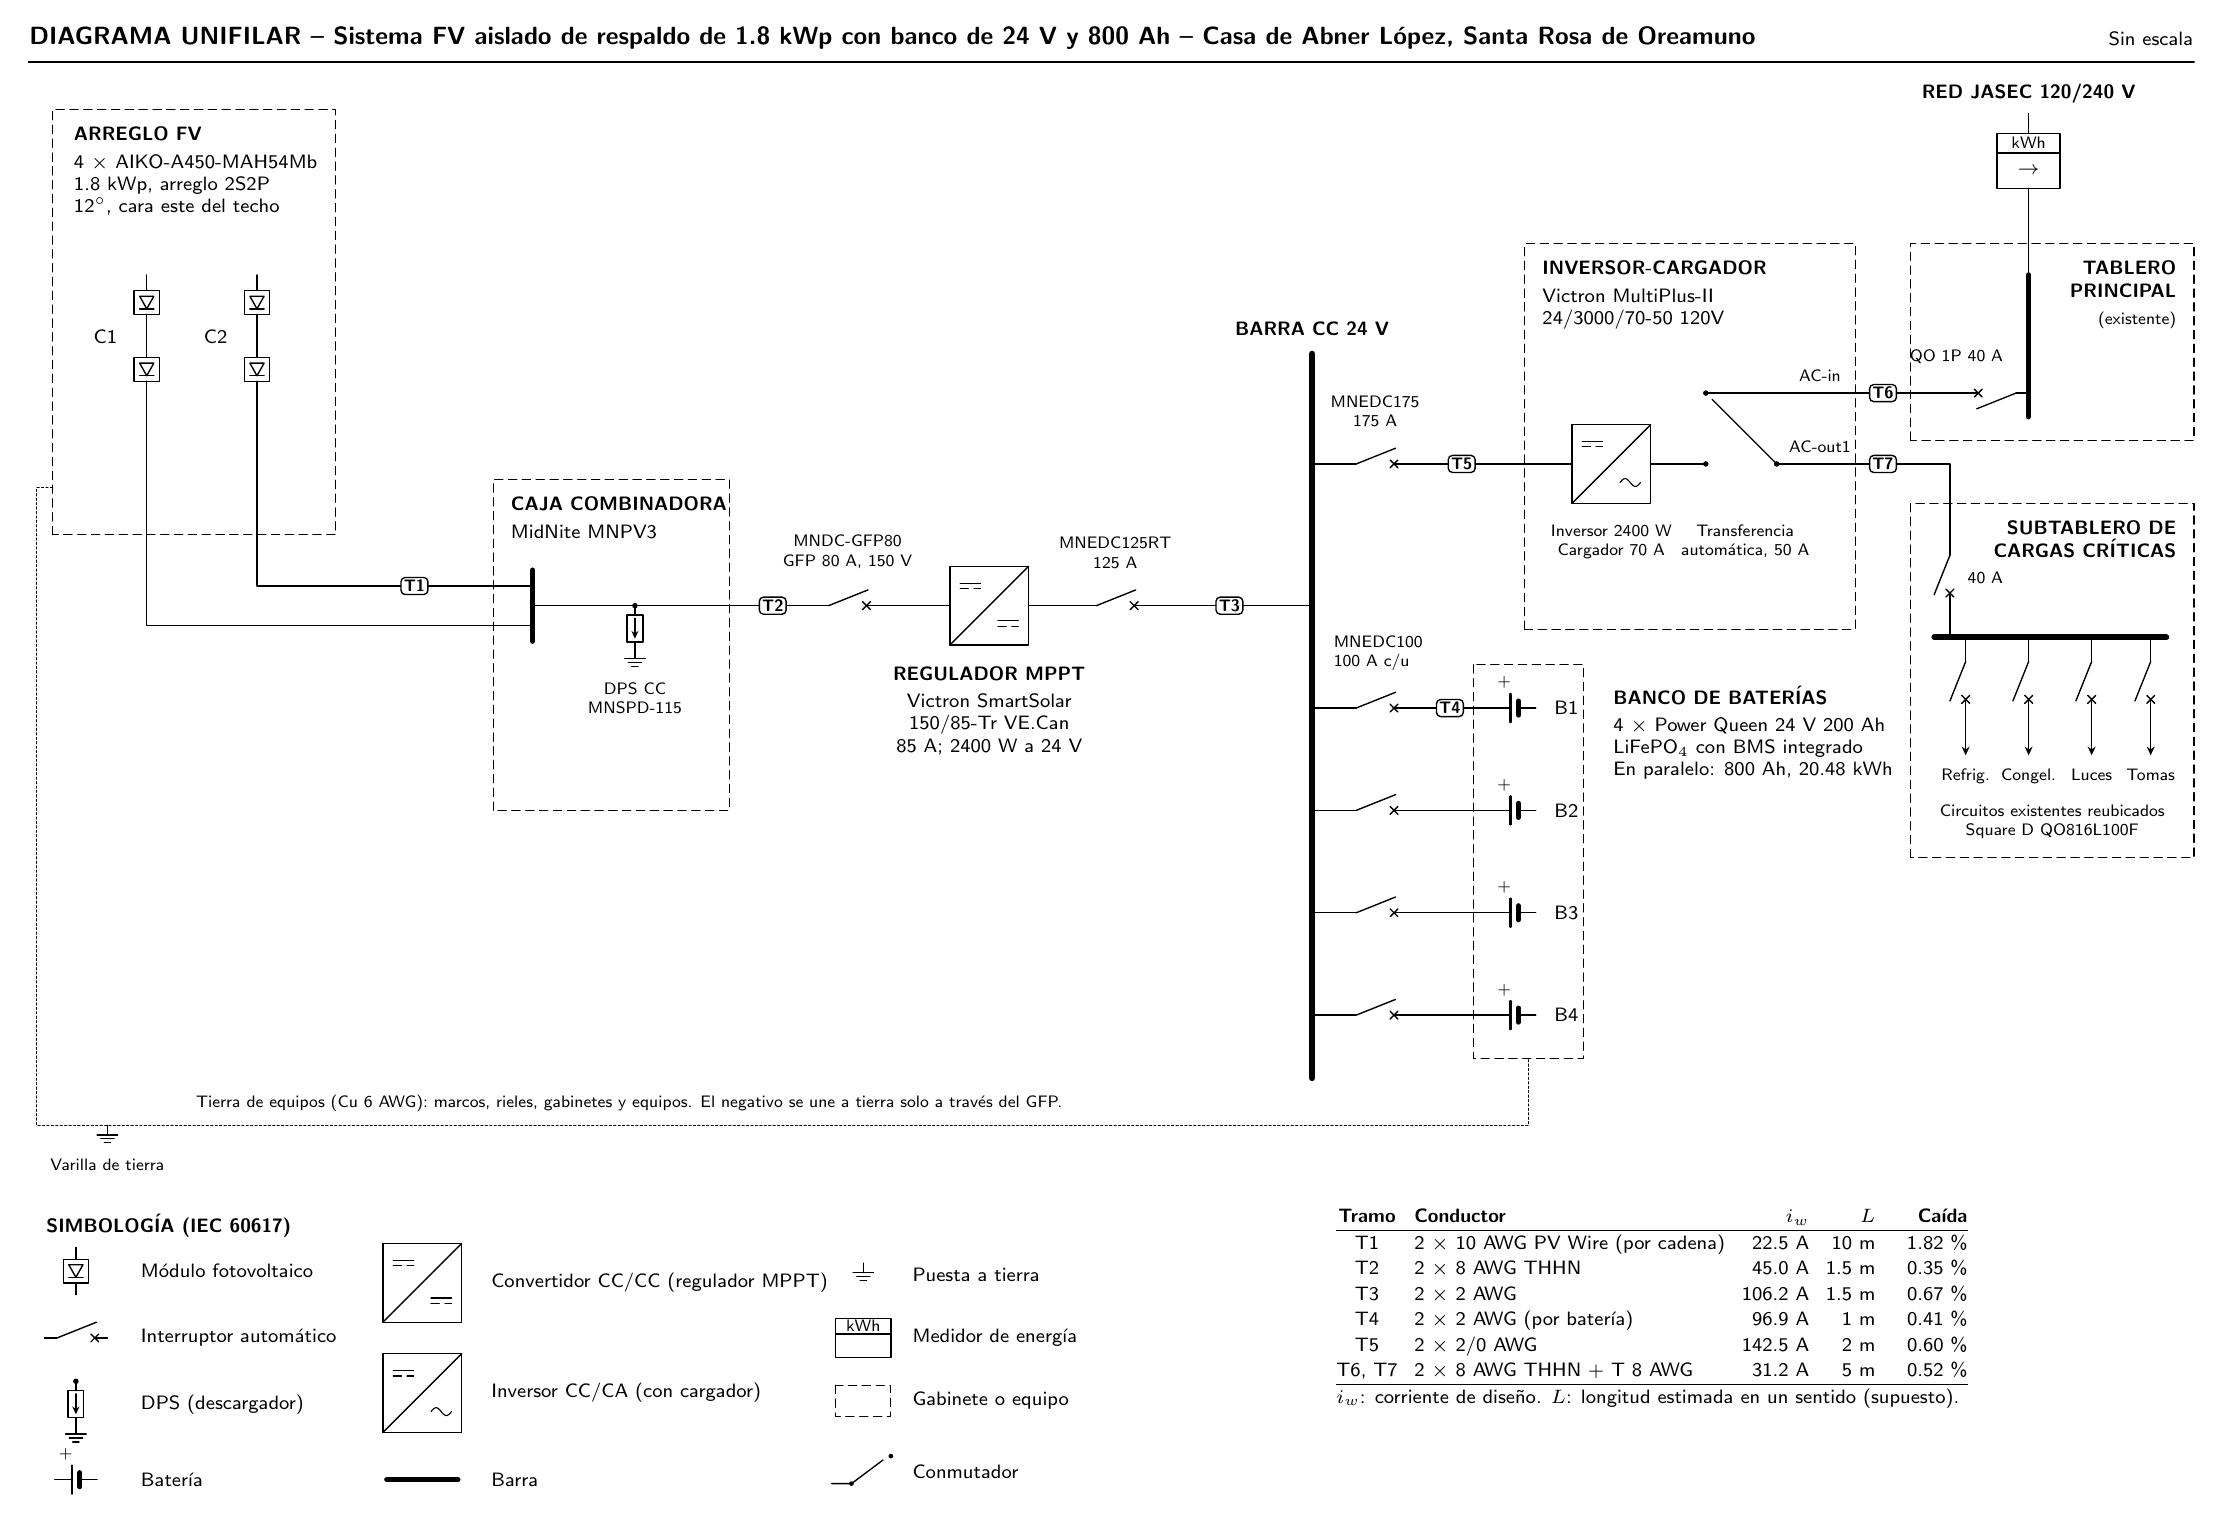
\begin{tikzpicture}[line width=0.5pt,line cap=round,line join=round]

% ================================================================ título
\node[Ft,anchor=west,inner sep=0] at (0,7.2) {DIAGRAMA UNIFILAR \textendash{} Sistema FV aislado de respaldo de 1.8 kWp con banco de 24 V y 800 Ah \textendash{} Casa de Abner López, Santa Rosa de Oreamuno};
\node[Fn,anchor=east,inner sep=0] at (27.5,7.2) {Sin escala};
\draw[line width=0.7pt] (0,6.9) -- (27.5,6.9);

% ================================================================ arreglo FV
\draw[enc] (0.3,0.9) rectangle (3.9,6.3);
\node[Fb,anchor=north west] at (0.45,6.2) {ARREGLO FV};
\node[Fn,anchor=north west,align=left] at (0.45,5.85) {4 $\times$ AIKO-A450-MAH54Mb\\1.8 kWp, arreglo 2S2P\\12$^\circ$, cara este del techo};
\foreach \x/\n in {1.5/C1,2.9/C2}{
  \draw (\x,4.0) -- (\x,4.2);
  \pic at (\x,3.85) {fv}; \draw (\x,3.7) -- (\x,3.15); \pic at (\x,3.0) {fv};
  \draw (\x,2.85) -- (\x,0.9);
  \node[Fn,anchor=east] at (\x-0.25,3.42) {\n};
}
% cadenas hacia la caja combinadora
\draw (2.9,0.9) -- (2.9,0.25) -- (6.2,0.25);
\draw (1.5,0.9) -- (1.5,-0.25) -- (6.2,-0.25);
\node[tag] at (4.9,0.25) {T1};

% ================================================================ caja combinadora
\draw[enc] (5.9,-2.6) rectangle (8.9,1.6);
\node[Fb,anchor=north west] at (6.0,1.5) {CAJA COMBINADORA};
\node[Fn,anchor=north west] at (6.0,1.15) {MidNite MNPV3};
\draw[line width=2pt] (6.4,-0.45) -- (6.4,0.45);
\draw (6.2,0.25) -- (6.4,0.25); \draw (6.2,-0.25) -- (6.4,-0.25);
\draw (6.4,0) -- (8.9,0);
\pic at (7.7,0) {dps};
\node[Fs,anchor=north,align=center] at (7.7,-0.85) {DPS CC\\MNSPD-115};

% ================================================================ T2 y protector de falla a tierra
\draw (8.9,0) -- (10.0,0);
\node[tag] at (9.45,0) {T2};
\pic at (10.0,0) {tm};
\node[Fs,anchor=south,align=center] at (10.4,0.35) {MNDC-GFP80\\GFP 80 A, 150 V};
\draw (10.8,0) -- (11.7,0);

% ================================================================ regulador MPPT
\pic at (12.2,0) {conv={\cc}{\cc}};
\node[Fb,anchor=north] at (12.2,-0.65) {REGULADOR MPPT};
\node[Fn,anchor=north,align=center] at (12.2,-1.0) {Victron SmartSolar\\150/85-Tr VE.Can\\85 A; 2400 W a 24 V};
\draw (12.7,0) -- (13.4,0);
\pic at (13.4,0) {tm};
\node[Fs,anchor=south,align=center] at (13.8,0.35) {MNEDC125RT\\125 A};
\draw (14.2,0) -- (16.3,0);
\node[tag] at (15.25,0) {T3};

% ================================================================ barra CC
\draw[line width=2.2pt] (16.3,3.2) -- (16.3,-6.0);
\node[Fb,anchor=south] at (16.3,3.3) {BARRA CC 24 V};

% ================================================================ banco de baterías
\foreach \y/\n in {-1.3/B1,-2.6/B2,-3.9/B3,-5.2/B4}{
  \draw (16.3,\y) -- (16.7,\y); \pic at (16.7,\y) {tm}; \draw (17.5,\y) -- (18.6,\y);
  \pic at (18.6,\y) {bath};
  \node[Fn,anchor=west] at (19.25,\y) {\n};
}
\node[Fs,anchor=south west,align=left] at (16.45,-0.95) {MNEDC100\\100 A c/u};
\node[tag] at (18.05,-1.3) {T4};
\draw[enc] (18.35,-0.75) rectangle (19.75,-5.75);
\node[Fb,anchor=north west] at (20.0,-0.9) {BANCO DE BATERÍAS};
\node[Fn,anchor=north west,align=left] at (20.0,-1.3) {4 $\times$ Power Queen 24 V 200 Ah\\LiFePO$_4$ con BMS integrado\\En paralelo: 800 Ah, 20.48 kWh};

% ================================================================ inversor-cargador
\draw (16.3,1.8) -- (16.7,1.8); \pic at (16.7,1.8) {tm};
\node[Fs,anchor=south,align=center] at (17.1,2.15) {MNEDC175\\175 A};
\draw (17.5,1.8) -- (19.6,1.8);
\node[tag] at (18.2,1.8) {T5};
\draw[enc] (19.0,-0.3) rectangle (23.2,4.6);
\node[Fb,anchor=north west] at (19.1,4.5) {INVERSOR-CARGADOR};
\node[Fn,anchor=north west,align=left] at (19.1,4.15) {Victron MultiPlus-II\\24/3000/70-50 120V};
\pic at (20.1,1.8) {conv={\cc}{\ca}};
\node[Fs,anchor=north,align=center] at (20.1,1.15) {Inversor 2400 W\\Cargador 70 A};
% conmutador de transferencia
\draw (20.6,1.8) -- (21.3,1.8); \fill (21.3,1.8) circle (0.035);
\fill (21.3,2.7) circle (0.035);
\fill (22.2,1.8) circle (0.035);
\draw (22.2,1.8) -- (21.38,2.62);
\draw (21.3,2.7) -- (23.2,2.7);
\draw (22.2,1.8) -- (23.2,1.8);
\node[Fs,anchor=south] at (22.75,2.72) {AC-in};
\node[Fs,anchor=south] at (22.75,1.82) {AC-out1};
\node[Fs,anchor=north,align=center] at (21.8,1.15) {Transferencia\\automática, 50 A};

% ================================================================ red y tablero principal
\node[Fb,anchor=south] at (25.4,6.25) {RED JASEC 120/240 V};
\draw (25.4,6.25) -- (25.4,6.0);
\draw[fill=white] (25.0,5.3) rectangle (25.8,6.0); \draw (25.0,5.75) -- (25.8,5.75);
\node[Fs] at (25.4,5.875) {kWh}; \node[Fn] at (25.4,5.52) {$\rightarrow$};
\draw (25.4,5.3) -- (25.4,4.2);
\draw[enc] (23.9,2.1) rectangle (27.5,4.6);
\node[Fb,anchor=north east,align=right] at (27.4,4.5) {TABLERO\\PRINCIPAL};
\node[Fs,anchor=north east] at (27.4,3.85) {(existente)};
\draw[line width=2pt] (25.4,4.2) -- (25.4,2.4);
\pic[rotate=180] at (25.4,2.7) {tm};
\node[Fs,anchor=south east] at (25.2,2.95) {QO 1P 40 A};
\draw (24.6,2.7) -- (23.2,2.7);
\node[tag] at (23.55,2.7) {T6};

% ================================================================ subtablero de cargas críticas
\draw (23.2,1.8) -- (24.4,1.8) -- (24.4,0.8);
\node[tag] at (23.55,1.8) {T7};
\draw[enc] (23.9,-3.2) rectangle (27.5,1.3);
\node[Fb,anchor=north east,align=right] at (27.4,1.2) {SUBTABLERO DE\\CARGAS CRÍTICAS};

\pic at (24.4,0.8) {tmv};
\node[Fs,anchor=west] at (24.5,0.35) {40 A};
\draw (24.4,0.0) -- (24.4,-0.4);
\draw[line width=2pt] (24.2,-0.4) -- (27.15,-0.4);
\foreach \x/\t in {24.6/Refrig.,25.4/Congel.,26.2/Luces,26.95/Tomas}{
  \draw (\x,-0.4) -- (\x,-0.55); \pic at (\x,-0.55) {tmv};
  \draw[-{Stealth[length=1.1mm,width=1mm]}] (\x,-1.35) -- (\x,-1.9);
  \node[Fs,anchor=north] at (\x,-1.95) {\t};
}
\node[Fs,anchor=north,align=center] at (25.7,-2.4) {Circuitos existentes reubicados\\Square D QO816L100F};

% ================================================================ puesta a tierra
\draw[densely dotted,line width=0.6pt] (0.3,1.5) -- (0.1,1.5) -- (0.1,-6.6) -- (19.05,-6.6) -- (19.05,-5.75);
\pic at (1.0,-6.6) {tierra};
\node[Fs,anchor=north] at (1.0,-6.9) {Varilla de tierra};
\node[Fs,anchor=south west] at (2.0,-6.55) {Tierra de equipos (Cu 6 AWG): marcos, rieles, gabinetes y equipos. El negativo se une a tierra solo a través del GFP.};

% ================================================================ simbología
\node[Fb,anchor=north west] at (0.1,-7.6) {SIMBOLOGÍA (IEC 60617)};
\pic at (0.6,-8.45) {fv}; \draw (0.6,-8.3) -- (0.6,-8.15); \draw (0.6,-8.6) -- (0.6,-8.75);
\node[Fn,anchor=west] at (1.3,-8.45) {Módulo fotovoltaico};
\pic at (0.2,-9.3) {tm}; \node[Fn,anchor=west] at (1.3,-9.3) {Interruptor automático};
\pic at (0.6,-9.85) {dps}; \node[Fn,anchor=west] at (1.3,-10.15) {DPS (descargador)};
\pic at (0.33,-11.1) {bath}; \node[Fn,anchor=west] at (1.3,-11.1) {Batería};
\pic at (5.0,-8.6) {conv={\cc}{\cc}}; \node[Fn,anchor=west] at (5.75,-8.6) {Convertidor CC/CC (regulador MPPT)};
\pic at (5.0,-10.0) {conv={\cc}{\ca}}; \node[Fn,anchor=west] at (5.75,-10.0) {Inversor CC/CA (con cargador)};
\draw[line width=2pt] (4.55,-11.1) -- (5.45,-11.1); \node[Fn,anchor=west] at (5.75,-11.1) {Barra};
\pic at (10.6,-8.35) {tierra}; \node[Fn,anchor=west] at (11.1,-8.5) {Puesta a tierra};
\draw[fill=white] (10.25,-9.05) rectangle (10.95,-9.55); \draw (10.25,-9.25) -- (10.95,-9.25);
\node[Fs] at (10.6,-9.15) {kWh}; \node[Fn,anchor=west] at (11.1,-9.3) {Medidor de energía};
\draw[enc] (10.25,-9.9) rectangle (10.95,-10.3); \node[Fn,anchor=west] at (11.1,-10.1) {Gabinete o equipo};
\draw (10.2,-11.15) -- (10.45,-11.15) -- (10.85,-10.85); \fill (10.45,-11.15) circle (0.03); \fill (10.95,-10.8) circle (0.03);
\node[Fn,anchor=west] at (11.1,-11.0) {Conmutador};

% ================================================================ tabla de conductores
\node[Fn,anchor=north west,inner sep=0] at (16.6,-7.6) {\begin{tabular}{@{}c l r r r@{}}\textbf{Tramo} & \textbf{Conductor} & $i_w$ & $L$ & \textbf{Caída}\\\hline
T1 & 2 $\times$ 10 AWG PV Wire (por cadena) & 22.5 A & 10 m & 1.82 \%\\
T2 & 2 $\times$ 8 AWG THHN & 45.0 A & 1.5 m & 0.35 \%\\
T3 & 2 $\times$ 2 AWG & 106.2 A & 1.5 m & 0.67 \%\\
T4 & 2 $\times$ 2 AWG (por batería) & 96.9 A & 1 m & 0.41 \%\\
T5 & 2 $\times$ 2/0 AWG & 142.5 A & 2 m & 0.60 \%\\
T6, T7 & 2 $\times$ 8 AWG THHN + T 8 AWG & 31.2 A & 5 m & 0.52 \%\\\hline
\multicolumn{5}{@{}l}{$i_w$: corriente de diseño. $L$: longitud estimada en un sentido (supuesto).}\end{tabular}};
\end{tikzpicture}
\end{document}
